\chapter{An IFR Cross Country Flight Tutorial\label{ifr}}

\section{Introduction}

\begin{figure}[h]
  \begin{center}
    \includegraphics[width=6cm]{img/somewhere}
    \caption{Flying over the San Antonio Dam to Livermore.  I think.}
    \label{fig:somewhere}
  \end{center}
\end{figure}

In the cross country flight tutorial, you learned about VFR flight,
and in the course of the flight you were introduced to most of the
flight instruments in the C172p.  Now we're going to do an Instrument
Flight Rules (IFR) flight.  In this flight you'll be introduced to the
remaining instruments, learn a bit about IFR flight, and learn many,
many TLAs (Three-Letter Acronyms).

We'll fly the same flight, from Reid-Hillview (KRHV), runway 31R, to
Livermore (KLVK), runway 25R, only this time we'll do it in IFR
conditions: a 750 foot ceiling, and 1 mile visibility.  This tutorial
assumes you've completed the cross country flight tutorial.

\subsection{Disclaimer}

This is not intended to teach you how to fly IFR.  Rather, it is meant
to give a flavour of what IFR flying is like, and remove the mystery
of the panel instruments not covered by the cross country flight
tutorial.

I'm not a pilot.  Like the previous tutorial, this information has
been gleaned from various non-authoritative sources.  If you find an
error or misunderstanding, please let me know.  Mail me at
bschack-flightgear -at- usa -dot- net.

\section{Before Takeoff}

We need to tell FlightGear about our flight conditions.  Depending on
which version of FlightGear you're using there are different ways to
set our ``desired'' weather.  You need to check your specific version
to see what you need to do.  In the command-line version, you need to
add the following options when you start up:

\begin{quote}
  \verb|--ceiling=750:3000 --visibility-miles=1|
\end{quote}

The first option asks for a 750 foot ceiling, with a thickness of 3000
feet (ie, the cloud tops are at 3750), the second should be obvious.
I strongly recommend also setting the following, admittedly hairy,
option:

\begin{quote}
  \verb|--prop:/environment/config/aloft/entry/visibility-m[0]=30000|
\end{quote}

% Note: we use the \string\ construct to insert backslashes into the
% footnote, where \verb doesn't work.

The option's not pretty,\footnote{In fact, you might have to make it
  even uglier, if you use csh or tcsh.  They'll complain about the
  square brackets, so you'll need to escape them:
  \ldots{}\texttt{visibility-m\string\[0\string\]}\ldots{}.  If you
  really don't like this, you can also set this option from the
  FlightGear menu: click \textbf{\textsf{Weather}} $\Rightarrow$
  \textbf{\textsf{Weather Conditions}}, and set the visibility in the
  3000 foot layer to 30000.} but the result is --- when you top out at
4000 feet, you'll be able to see for miles (30,000 metres, in fact),
including a few peaks poking through the clouds (without this option,
you'd have 1 mile visibility above the clouds as well as below them).
It's a small thing, and not strictly necessary, but there's something
very uplifting about rising above the clouds into a bright sunny
world, with blue sky above and a carpet of white below, like Figure
\ref{fig:somewhere}.

% Porco Rosso!

% Note: If I change the visibility while cruising, the autopilot
% momentarily spazzes.  What's with that?

% What are VFR minimums?  3 miles visibility, and basically 1000'
% ceiling (actually, 500 feet below the clouds, and since the minimum
% flight altitude is 500 feet AGL, that means at least 1000.
% Furthermore, you need to clear obstacles near cities by 1000 feet,
% so near cities, you need 1500' AGL).

% EYE - we need to create real references to the Cross Country Flight
% Tutorial.

\begin{figure}
  \begin{center}
    \includegraphics[width=10cm]{img/KRHV}
    \caption{On the runway at KRHV}
    \label{fig:KRHV}
  \end{center}
\end{figure}

\subsection{Flight Planning}

Unfortunately, when you start, you won't see a carpet of white.
You'll see something more like Figure \ref{fig:KRHV}.  Those clouds
don't look very friendly, and it's hard to even see past the end of
the runway.  Maybe we should just \emph{drive} there in the Cessna.
We had been planning to practice ground steering anyway \ldots{}

So how do you get from A to B when you can't see?  There are a variety
of ways that have evolved over the years, with various advantages and
disadvantages.  Our flight will use all of the navigation instruments
the standard Cessna C172p has, just to give a taste of what's
possible.

Our entire route, and the aids we'll be using, are shown in
Figure \ref{fig:sectional_labelled}.  Our route is in green, the
navigational aids blue and red.  The route looks a bit crazy --- in
fact, you might wonder if we're \emph{more} lost using our fancy
equipment than just flying by the seat of our pants --- but there is a
method to the madness.  Rather than overwhelming you with details by
explaining it all now, I'll explain it bit by bit as we go along.

\begin{figure}
  \begin{center}
    \includegraphics[width=20cm, angle=-90]{img/sectional_labelled}
    \caption{Green: our route, Blue: VORs and radials, Red: NDBs}
    \label{fig:sectional_labelled}
  \end{center}
\end{figure}

% IFR sectionals?

\subsection{VHF Omnidirectional Range}

The first bit will involve
VOR\footnote{See \url{http://en.wikipedia.org/wiki/VHF_omnidirectional_range}
for more information.} (VHF (Very High Frequency) Omnidirectional
Range) navigation, and will get us to a point about 5 nm (nautical
miles) south of Livermore.

VOR stations are indicated on the sectional by a big bluish-green
circle with compass markings around the outside.  I've helped you by
marking their centers with a big blue dot as well.  Reid-Hillview is
very close to one, San Jose, which you can see in Figure
\ref{fig:sectional_labelled}.  Near the centre of the circle, in a
bluish-green rectangle, is the station information.  According to the
station information, it's a VOR-DME station (I'll explain DME later),
its name is San Jose, its frequency is 114.1 MHz (or Channel 88, which
is an alternative way to say the same thing), and its identifier, or
``ident'', is SJC (which in Morse code is \mdot\mdot\mdot\mspace
\mdot\mdash\mdash\mdash\mspace \mdash\mdot\mdash\mdot).

% In emacs, try M-x morse-region on SJC
% .../.---/-.-.

To tune into a VOR station, we use one of the NAV receivers, which are
paired with the COMM receivers (see Figure \ref{fig:panel}).  And we
navigate using the corresponding VOR gauge.  We'll choose the NAV1
receiver (and VOR1 gauge) in this case (NAV2 would have worked just as
well).  Before setting the frequency, check out the VOR1 gauge.  It
should look like VOR1 in Figure \ref{fig:panel}.  The important thing
is the red and white flag.  That means there's no VOR signal, so we
can't trust the gauge.

\begin{figure}
  \begin{center}
    \includegraphics[width=12cm]{img/panel_labelled}
    \caption{IFR navigation Instruments}
    \label{fig:panel}
  \end{center}
\end{figure}

The NAV receiver has an active frequency, a standby frequency, and a
tuning knob, just like the COMM receiver.  Tune it to 114.1, and press
the swap button.  If you look at VOR1, you should notice that the red
and white flag has disappeared, to be replaced with a ``TO'' flag, as
in Figure \ref{fig:VOR1}.  That means we're receiving a signal.  But
is it the correct one?  What if we accidentally set the wrong
frequency?  What if there's a different VOR nearby with the same
frequency?

\begin{figure}
  \begin{center}
    \includegraphics[width=6cm]{img/VOR1}
    \caption{VOR1, after tuning}
    \label{fig:VOR1}
  \end{center}
\end{figure}

To confirm that we're tuned into the correct VOR, we listen for its
ident.  If you can't hear the ident, or if it doesn't match the chart,
don't trust the needle.  So far, you probably haven't heard a thing.
That seems strange.  After all, the red and white flag turned off.  We
must be in range of \emph{some} station, right?  Why can't we hear
anything?

When in doubt, look for the simplest solution.  In this case, check
the volume.  There's an extra dial on the NAV receivers that the COMM
receivers don't have, labelled OFF, LO, and HI (see Figure
\ref{fig:ident}).  That's our ident volume control.  So, is it
currently off, or low, or high?  Unfortunately, it gives no visual
feedback about its current state, so we don't really know.  The only
way to be sure is to turn it up.  Unfortunately, for the same reason,
it's hard to tell if our mouse clicks are doing any good, so hit
Ctrl-C to see the hot-spots.  This control has two hot-spots, one on
the top which increases the volume, the other on the left which
decreases it.  Increase the volume.  \emph{Now} you should hear the
ident: \mdot\mdot\mdot\mspace \mdot\mdash\mdash\mdash\mspace
\mdash\mdot\mdash\mdot.  Phew.

% SJC = .../.---/-.-.

\begin{figure}
  \begin{center}
    \includegraphics[width=6cm]{img/ident_knob}
    \caption{Ident volume knob and hot-spots}
    \label{fig:ident}
  \end{center}
\end{figure}

% EYE - \circ is ugly in \emph{}!  I need a real degree symbol!
Back to VOR1.  There's a knob labelled OBS (Omni Bearing Selector).
As the name vaguely suggests, it is used to select a bearing.  If you
turn it, you should see the vertical needle, called the CDI (Course
Deviation Indicator) move.\footnote{The horizontal needle is used in
  ILS landings, which will be explained later.}  Try to center the
needle.  It should center when the little arrow at the top points to
somewhere around 277.  That number, and the TO flag means: ``Flying at
a heading of \emph{277$^\circ$} will lead you directly \emph{to} the
station''.

That's great, except, according to our route, we don't want to go
\emph{to} the station.  We actually want to intercept the light blue
line labelled ``009$^\circ$'' (the ``9 degree radial'') coming
\emph{from} the station.  How do we do that?  Simple.  Set the OBS to
9.  When we fly across the radial, the needle will center, and the
flag will say FROM.  This tells us: ``flying at a heading of
\emph{9$^\circ$} will lead you directly away \emph{from} the
station'', which is what we want.  At that point we'll turn right to a
heading of 9$^\circ$.

One final thing --- set the heading bug on the directional gyro to our
current heading (about 310$^\circ$).

\subsection{Takeoff}

Now we're ready to take off.  It took a long time to get ready, but in
fact there's really more that we should have done.  For example, there
are all the things mentioned in the previous cross country flight
tutorial.  And there are other IFR preparations that we should have
made.  But again, in the interests of not overwhelming your brains,
I'm feeding out the information in trickles.  This brings us to the
most important control you have --- the `p' key.  Use this often,
especially when a new concept is introduced.

Okay.  Now take off, keeping a heading of 310$^\circ$ for now.  Establish a
steady rate of climb.  We plan to climb to 4000 feet.  There's just
one problem though --- those ugly looking clouds are standing in our
way.

\section{In the Air}

If this is your first attempt at IFR flight, you will find it nearly
impossible to fly once you enter the clouds.  When you enter the
clouds, you will be momentarily disconcerted by the lack of visual
cues.  ``No matter,'' you then think.  ``I'll just keep things
steady.''  In a few moments, though, you'll probably notice dials and
needles spinning crazily, and without knowing it, you'll be flying
upside down, or diving towards the ground, or stalling, or all three.

It takes practice to get used to flying without external visual clues,
although it's a skill that you definitely \emph{must} master if you
want to fly IFR.  For now though, we'll use ``George'', the autopilot,
to make this part of flying easier.

\subsection{George I}

Once you've established a steady rate of climb and heading, engage the
autopilot by pressing the AP button.  You should see ``ROL'' displayed
on the left to show that it's in ``roll mode'' --- it is keeping the
wings level.  In the middle it will display ``VS'', to show it is in
``vertical speed'' mode --- it is maintaining a constant vertical
speed.  On the right it will \emph{momentarily} display that vertical
speed (in feet per minute).  Initially, the value is your vertical
speed at the moment the autopilot is turned on.  In the case of
Figure \ref{fig:ap_vs}, the autopilot has set the vertical speed to
300 feet per minute.

\begin{figure}
  \begin{center}
    \includegraphics[width=7cm]{img/ap_vs}
    \caption{Autopilot after engaging}
    \label{fig:ap_vs}
  \end{center}
\end{figure}

% EYE - is it a bug?

When you engage the autopilot, CHECK THIS CAREFULLY.  Sometimes the
autopilot gets a very funny idea about what your current rate of climb
is, like 1800 feet per minute.  Our little Cessna cannot sustain this,
and if the autopilot tries to maintain this (and it will), you will
stall before you can say ``Icarus''.  This is a bug, to be sure, and a
bit annoying, but it is also a useful cautionary lesson --- don't put
blind faith in your equipment.  Things fail.  You have to monitor and
cross-check your equipment, and be prepared to deal with problems.

We want a vertical speed of around 500 to 700 feet per minute.  Hit
the up and down (UP and DN) buttons to adjust the vertical speed to a
nice value.  Take into account the airspeed as well.  We want a
sustainable rate of climb.

Finally, once you're climbing nicely, hit the heading (HDG) button.
On the display, ``ROL'' will change to ``HDG'', and the autopilot will
turn the airplane to track the heading bug.  Since you set the heading
bug to the runway heading, and you took off straight ahead (didn't
you?), it shouldn't turn much.

\subsection{MISON Impossible}

It's around 8 nm to the 009 radial intercept, so we've got a bit of
time.  Since there's no scenery to admire, we might as well prepare
for the next phase of the flight.

\begin{figure}
  \begin{center}
    \includegraphics[width=6cm]{img/murk}
    \caption{Typical IFR scenery}
    \label{fig:murk}
  \end{center}
\end{figure}

If you look along our route, just after we intercept the 009 radial
and turn north, we pass by a point labelled MISON (see Figure
\ref{fig:Oakland} for a closeup of that section of the chart without
my fat blue and green lines drawn on top.  MISON is in the lower
right).  Just above and to the left of MISON are two crossed arrows.
MISON is an intersection.  We're actually going to pass east of MISON,
but the radial passing roughly from northwest to southeast through
MISON (and our route) is of interest to us.  We're going to use it to
monitor our progress.

\begin{figure}
  \begin{center}
    \includegraphics[width=10cm]{img/Oakland}
    \caption{Oakland VOR and 114 radial to MISON intersection}
    \label{fig:Oakland}
  \end{center}
\end{figure}

Noting our passage of that radial isn't strictly necessary --- we can
just keep flying along the 009 radial from San Jose until we need to
turn.  But it's useful for two reasons: First, it's nice to know
exactly where we are.  Second, it confirms we are where we think we
are.  If we fly and fly and never cross the radial, alarm bells should
start going off.

% 009 or 9?

Looking at the sectional, we see that the radial is the 114 radial
from the Oakland VORTAC (VOR TACAN, where TACAN stands for Tactical
Air Navigation).  Oakland's frequency is 116.8, and its ident is OAK
(\mdash\mdash\mdash\mspace \mdot\mdash\mspace \mdash\mdot\mdash).
NAV2 should already be tuned to Oakland, but if it isn't, do it now.
Turn on NAV2's volume and make sure you're getting the correct ident.

% OAK = ---/.-/-.-

When we were on the ground, VOR2's needle was flickering --- VOR
signals are line-of-sight, and Oakland was too far away (and behind
some hills) for us to receive it clearly.  Soon after taking off,
however, it should have settled down, and now it should be holding
steady.

We need to adjust the OBS, to tell VOR2 which radial we're interested
in.  Set the OBS to 114.  See if you can guess whether the flag should
read TO or FROM when we cross the 114 radial.  And see if you can
guess whether the needle will move from left to right or right to left
as we cross the radial.

A final note: There's nothing magical about the 114 radial --- we
could have used 113, or 115, or 100, or 090.  The reason I chose 114
is because there was a line on the map already drawn along the 114
radial, which saved me the trouble of drawing a line myself.

\subsection{George II}

As we continue towards the 009 radial intercept, let's look a bit more
closely at the autopilot.  First of all, if you aren't in the habit of
trimming the airplane, you'll probably notice a flashing ``PT'' with
an arrow on the autopilot.  The autopilot is telling you to adjust the
pitch trim.  I tend to ignore it because, flying with a mouse,
trimming is more trouble than it's worth.  Those of you lucky people
with yokes and joysticks and who find flashing lights annoying might
want to trim to get rid of it.

Also, on the right there's a big knob, the altitude select knob, which
we can use to dial in a target altitude.  We're going to use it.  Turn
it until you see our desired cruising altitude, 4000 feet, displayed
on the right.  When you started turning it, ``ALT ARM'' should have
appeared in the autopilot display (as in Figure \ref{fig:ap_alt}).
This indicates that you've selected a target altitude.  The autopilot
will maintain the current rate of climb until reaching that altitude,
at which point it will level off and change from vertical speed (VS)
mode to altitude hold (ALT) mode.  In altitude hold mode it maintains
an altitude (in this case our target altitude of 4000 feet).\footnote{
  Of course, you don't really have to do this --- you could just watch
  the altimeter, and when it gets to 4000 feet, reduce the vertical
  speed to 0, or press the ALT button to enter altitude hold mode.
  But by using the altitude select knob, we've demystified one more
  mystery button.}

\begin{figure}
  \begin{center}
    \includegraphics[width=7cm]{img/ap_alt}
    \caption{Autopilot with altitude armed}
    \label{fig:ap_alt}
  \end{center}
\end{figure}

Don't forget that the autopilot won't adjust the throttle, so when it
levels out, the airplane (and engine) will speed up to potentially
dangerous levels.  You'll need to adjust the throttle to get a proper
cruise.

\subsection{Staying the Course}

I assume by this point you've turned onto the 009 radial.  Unless
you're good or lucky, the needle probably won't be centered.  We need
to adjust our course.  The CDI needle (the vertical needle on the VOR)
tells us where to go.  If it's to the left, that means the radial is
to the left, so we need to go left.  Ditto for right.

It's quite easy in theory, although in practice you may find that it's
hard to keep the needle centered, and that you are slaloming down the
radial.  The key is to realize this: the \emph{position} of the needle
tells us where we \emph{are}, the \emph{motion} of the needle tells us
what to \emph{do}.

I'll explain.  If the needle is to our left, then, yes, the radial is
definitely to our left.\footnote{Unless you're heading in the opposite
  direction, but that's another story.}  But if the needle is
\emph{moving} towards us, that means we're going to cross the radial,
sooner or later, so our situation is improving, and we probably just
need to wait for the needle to center.  On the other hand, if the
needle is \emph{moving} away, we need to turn towards it to stop, and
reverse, its motion.

Note that the amount we need to turn is difficult to guess correctly
at first, so experiment.  Try 10$^\circ$.  If the needle moves too
fast, cut it down to 5$^\circ$ (ie, turn back 5$^\circ$).  If, on the
other hand, the needle moves too slowly, double it to 20$^\circ$ (ie,
add another 10$^\circ$), and see what happens.

\subsection{Yet More Cross-Checks}

Cross-checking your position is always a good thing.  The intersection
with the Oakland 114 radial was one way (I assume that by now you've
crossed it).  Ahead of us lies the SUNOL intersection.  If you look
closely, 5 separate radials join at the point, so we have an
embarrassment of choices with regards to the intersecting radial.
Because it will come in useful later, we're going to use the one
coming in from the upper right.  Another check of the sectional
reveals that this is the 229 radial of the Manteca VOR, 116.0 MHz,
ident ECA (\mdot\mspace \mdash\mdot\mdash\mdot\mspace \mdot\mdash).

% ECA = ./-.-./.-

You should know the drill by now: Tune NAV2 to 116.0, set the OBS to
229, and check the ident to confirm the station.

Meanwhile, let's introduce another piece of gear on the panel that
will cross-check the SUNOL passage.  Some VOR stations have a distance
capability, called DME\footnote{See
  \url{http://en.wikipedia.org/wiki/Distance_Measuring_Equipment} for
  more information.} (Distance Measuring Equipment).  For example, San
Jose does (remember it's a VOR-DME station), as does Oakland (VORTAC
also means it has DME capabilities).  It turns out Manteca does as
well.

Using DME, you can find out how far you are, in straight-line
distance, from the VOR station.  In our scenario, the DME isn't
necessary, but we'll use it anyway, just to see how it works, and to
reconfirm our position.

The DME is the instrument below the autopilot (refer to Figure
\ref{fig:panel}).  Probably the selector is set to N1.  The N1 means
``listen to NAV1'', and since NAV1 is tuned to San Jose, it's telling
us the distance to the San Jose VOR-DME.  Now switch the DME to N2.
It now shows us the distance to the Manteca VOR.

The DME shows you 3 things: the distance in nautical miles to the
station, your speed towards or away from the station, and estimated
time to the station at the current speed.  Note that the distance is
the direct distance from your plane to the station (called the ``slant
distance''), not the ground distance.  Note as well that the speed is
relative to the station, so unless you're flying directly to or from
the station, it will probably be lower than your true groundspeed.
For example, the speed from San Jose, which is directly behind us,
should be greater than the speed towards Manteca, which is off to the
right.

If we look up information about the SUNOL intersection,\footnote{For
  example, from \url{http://www.airnav.com/airspace/fix/SUNOL}.} it
tells us that it is 33.35 nm (as measured by a DME receiver) from ECA
on the 229.00 radial (that's what ``ECAr229.00/33.35'' means).

Now we have two ways to confirm the SUNOL intersection: The VOR2
needle will center, and the DME will read 33.4 or so.  Note that the
DME doesn't provide us with a very precise fix here because Manteca is
at such an oblique angle.  But it does give us a good warning of
SUNOL's impending arrival.  Moreover, if it has an unexpected value
(like 30), it should raise a few alarm bells.

% EYE - acronym, then expansion, or vice-versa?

You may be wondering what ``HLD'' means (the setting between N1 and N2
on the DME).  It stands for ``hold'', and means ``retain the current
frequency, regardless of whether NAV1 or NAV2 are retuned''.  For
example, if we switch from N2 to HLD, the DME will continue to display
(and update) information to Manteca.  Even if we retune NAV2, the DME
will remain tuned to Manteca.  This is handy, because it basically
represents a third independent receiver, and in IFR flight two
receivers just never seem like enough.

% Does C172p have an audio panel?  How can we hear the ident for the
% DME?  And how do we switch between COMM1 and COMM2?

\section{Getting Down}

We're getting close to SUNOL, flying along the 009 radial from San
Jose, monitoring our position with the DME.  At SUNOL we'll be less
than 5 nm from Livermore, somewhere down there in the clouds.  Perhaps
if we just descended to 700 feet or so (Livermore is at 400, the
ceiling is at 750) and headed more or less directly north after SUNOL,
we'd get there?  A recipe for disaster my friend, and you know it.

\subsection{Instrument Approach Procedures}

As you recall from the previous tutorial, when flying VFR, you don't
just point your airplane to the nearest runway to land.  You need to
fly a pattern.  This helps you line up, and helps prevent planes from
crashing into one another, which is a Good Thing.

Similarly with IFR landings.  There's a procedure to follow.  In fact,
there are \emph{procedures} to follow.  Because of the complexity of
landing in IFR conditions, there's no single procedure for all
airports.  You need to check for your particular airport.  In fact,
you usually need to check for your particular airport, runway, and
navigation equipment.

Our airport is Livermore (KLVK).  Let's check the information for that
airport.  Go to \url{http://www.airnav.com/airport/KLVK} to see what
they've got.  Down near the bottom, we have IAPs (Instrument Approach
Procedures).  There are two listed for runway 25R.  One is an ILS
(Instrument Landing System) approach, the other a GPS (Global
Positioning System) approach.  Our plane has no GPS, but it does have
ILS capabilities (I'll explain ILS later), so we'll choose that.

Although Livermore only has two different instrument approach
procedures, big airports have many many more.  If you look at nearby
San Francisco, you'll see they have a \emph{slew} of procedures.
There are ILS procedures, GPS procedures, LDA procedures, VOR
procedures, \ldots{} I wouldn't be surprised if they had a procedure
for someone with a sextant and an hourglass in there.  To learn IFR
flight, you'll need to master all of them.

Back to Livermore.  If you download the procedure, you'll see
something like Figure \ref{fig:big_plate} (except for the colour).
It's pretty overwhelming at first --- it compresses a lot of
information in a small space.  We'll ignore as much as we can,
restricting ourselves to the three parts that have been coloured in.
And we'll do those parts on a ``need to know'' basis --- we'll only
look at them when we really have to.

\begin{figure}
  \begin{center}
    \includegraphics[width=14cm]{img/big_plate}
    \caption{ILS approach plate for Livermore runway 25R}
    \label{fig:big_plate}
  \end{center}
\end{figure}

Where to start?  At the beginning of course.  An IAP will have one or
more Initial Approach Fixes (IAFs).  These are your entry points to
the approach procedure and can be found in the ``plan view'', which
I've coloured purple in Figure \ref{fig:big_plate}.  Our IAP lists
two, one in the middle and one on the right (see Figure \ref{fig:IAFs}
for a close-up).

\begin{figure}
  \begin{center}
    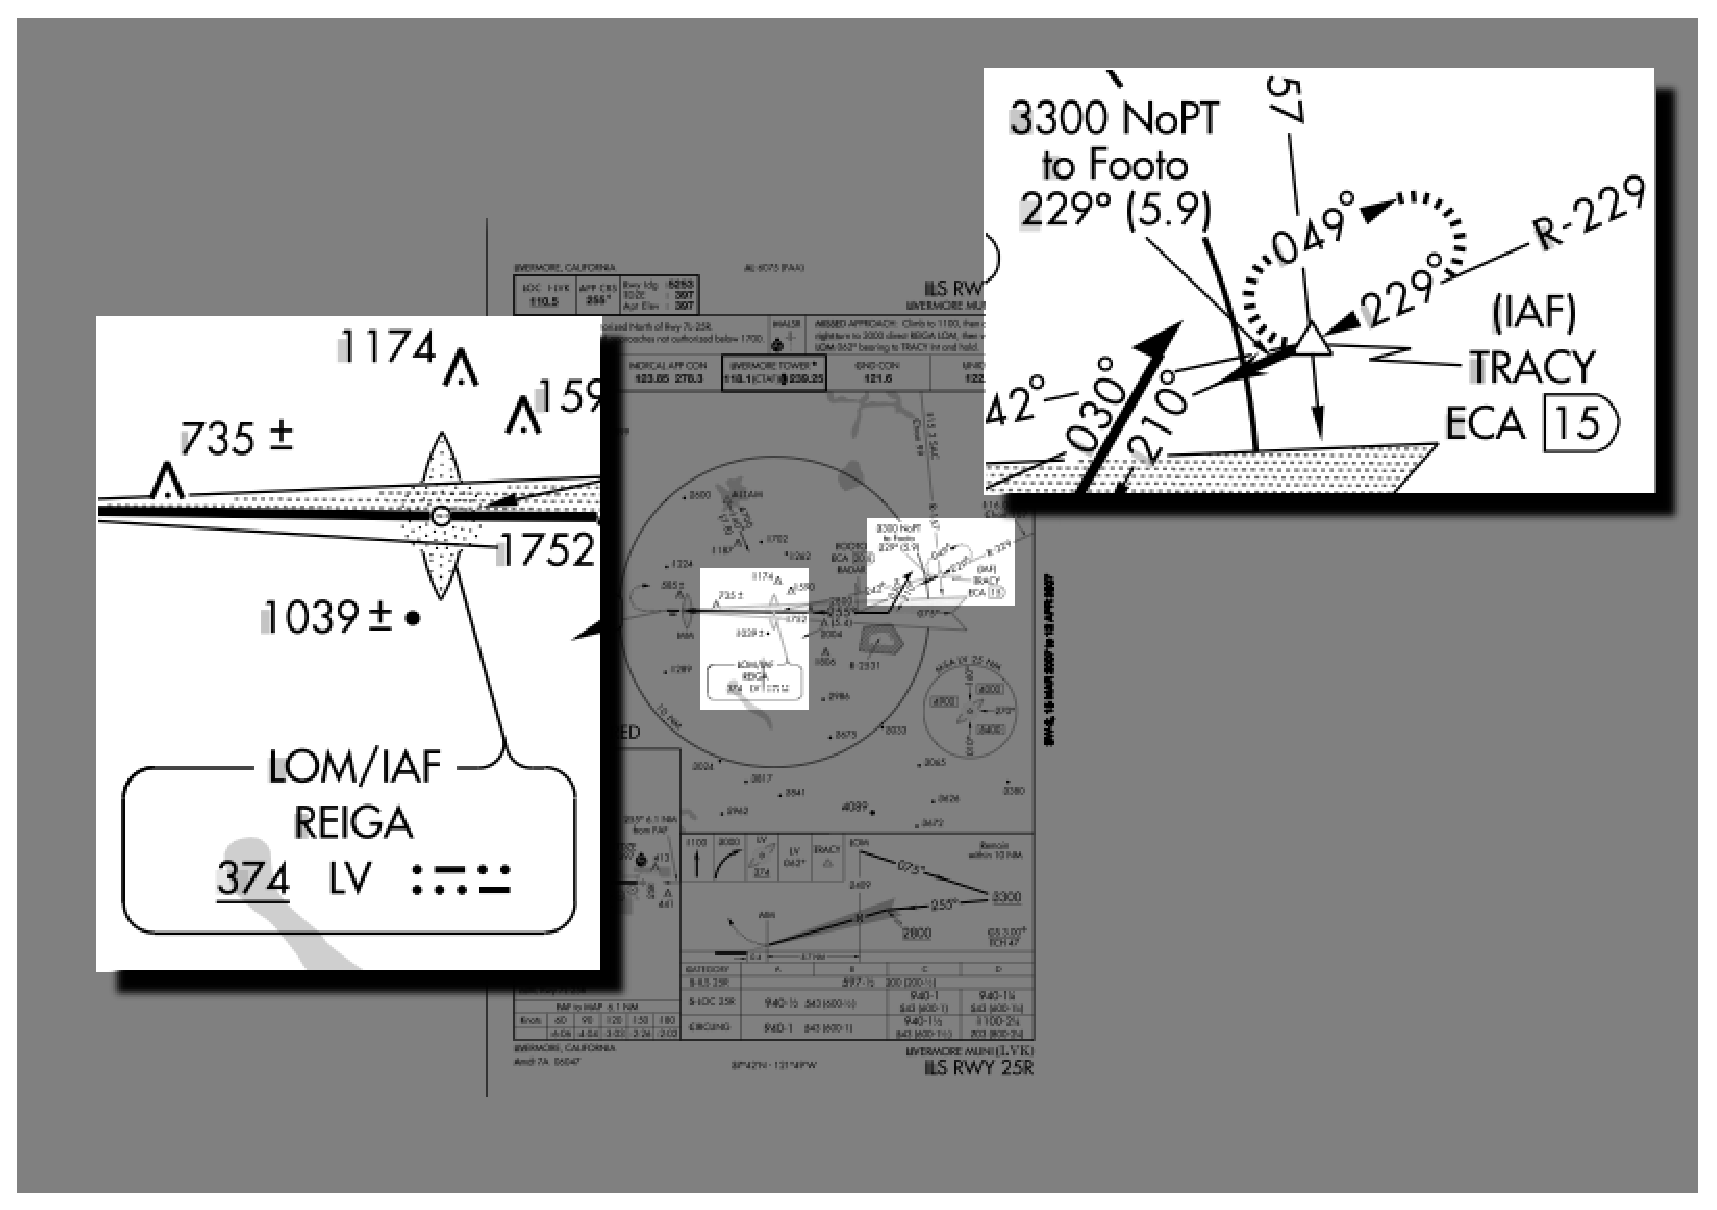
\includegraphics[width=10cm]{img/IAFs}
    \caption{Initial approach fixes}
    \label{fig:IAFs}
  \end{center}
\end{figure}

% EYE - is the altitude important?

An IAF is a \emph{fix}, and a fix is an identifiable point in space.
In fact, we've already encountered another kind of fix, namely a VOR
intersection.  Fixes are also usually named (eg, MISON, SUNOL).  The
IAF on the right is named TRACY, and consists of a radial, a distance,
and an altitude.  Specifically, it's 15 DME (15 nm as measured by a
DME receiver) along the 229 radial from the ECA (ie, Manteca) VOR.

% , at an altitude of 3300 feet.

% Notice that I said 15 DME, which means the distance in nautical
% miles as reported by a DME.  This is usually different than ground
% distance.  Notice as well we need an altitude --- the distance
% reported by the DME is straight-line distance to your plane, and so
% your height makes a difference.

\subsection{Nondirectional Beacons}

However, we're not going to use TRACY as our IAF.  We're going to use
the IAF in the middle, which is a marker (LOM stands for ``Locator
Outer Marker'').  We'll worry about what an outer marker is later.
For now let's concentrate on the locator part.  The locator in an LOM
is an NDB\footnote{See
  \url{http://en.wikipedia.org/wiki/Non-directional_beacon} for more
  information.} (nondirectional beacon).  It's a bit like a VOR, in
that it can be used to determine your heading and navigate from place
to place.  Like a VOR, it has a name (REIGA, in this case), a
frequency (374 kHz), and an ident (LV, or
{\mdot\mdash\mdot\mdot\mspace \mdot\mdot\mdot\mdash} in Morse).  NDBs
also appear on sectionals, as fuzzy red circles with a small circle in
the middle, with their identification information placed in a red box
nearby. (see Figure \ref{fig:NDB} for a closeup.  Don't confuse the
NDB, which is fuzzy, with the solid red circle on the left, nor the
circle below with the ``R'' inside).

% LV = .-../...-

\begin{figure}
  \begin{center}
    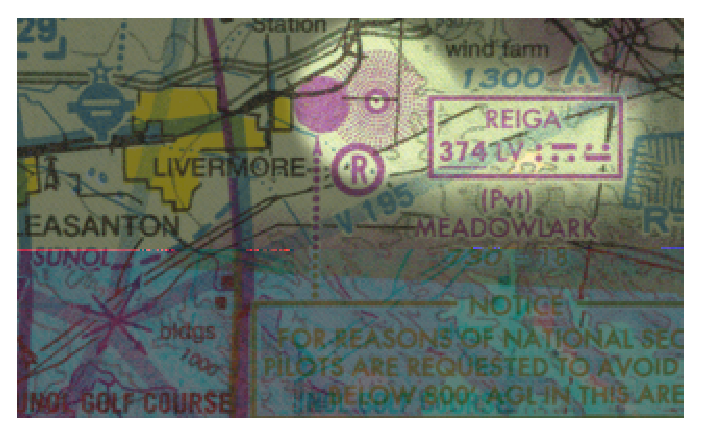
\includegraphics[width=8cm]{img/NDB}
    \caption{REIGA nondirectional beacon}
    \label{fig:NDB}
  \end{center}
\end{figure}

An NDB station basically broadcasts a signal that says ``I'm over
here'', and the receiver on the plane can receive that signal and tell
you, the pilot, ``the station is over there''.  You just need to tune
the receiver and monitor the correct instruments.  The receiver,
labelled ADF (Automatic Direction Finder), and the corresponding
instrument, also labelled ADF, are shown in Figure \ref{fig:panel}.

To tune into REIGA, turn the tuning knob on the receiver until 374 is
displayed as the standby (STDBY) frequency.  As usual, use the middle
mouse button for big changes (100 kHz in this case), and the left
mouse button for small changes (1 kHz).  Then hit the SWAP button.
The 374 is now displayed as the selected (SEL) frequency.  The needle
on the ADF should swing around, eventually pointing ahead to the
right.  This shouldn't be too surprising, since that's about where the
REIGA NDB is.  Like VORs, to be sure we're really tuned into the right
station, we need to hear the ident as well.

Unlike the NAV receivers, the ADF receiver has a dedicated IDENT
switch.  Turn it on, and wait a bit.  You should hear something.  If
you don't, though, it's possible that the volume is turned off.  Turn
the ADF volume up to high (the ADF volume switch works the same as the
NAV volume switch, with the same problems).  If you still can't hear
the ident, you've either dialled in the wrong frequency, you haven't
waited long enough, or you're really, really lost.

Notice there's no OBS to set for an ADF --- the needle just points to
the station, which is nice.  This leads us to our first rule for ADFs:

\begin{quote}
  \begin{description}
  \item[ADF Rule 1:] The needle points to the station.
  \end{description}
\end{quote}

Pretty simple.  In fact, you may not think it merits a ``rule'', but
it's important to emphasize the difference between ADFs and VORs.  A
VOR, remember, tracks a single radial, which you specify by turning
the OBS.  An ADF has a knob, and a identical-looking compass card, so
it's tempting to believe it acts the same way.  It doesn't.  Turn the
ADF heading knob and see what happens.  The compass card moves, but
the arrow doesn't.  It just \emph{points to the station}.

In our current situation, where we just want to fly to REIGA, that's
all we need to know to use the ADF.  If the needle points ``over
there'', then we'll fly ``over there'', and eventually we'll pass over
REIGA.  However, for the sake of practice, and because it will be
necessary later, I'm going to give the second rule for ADFs, which
explains what the compass card is there for:

\begin{quote}
  \begin{description}
  \item[ADF Rule 2:] \emph{If} the compass card reflects our current
    heading, then the needle gives the bearing \emph{to} the station.
  \end{description}
\end{quote}

In other words, the compass card gives ``over there'' a number.

% EYE - heading vs bearing vs track vs course
% heading: where your nose is pointed
% bearing: a radial
% tracking (v): compensating for wind to fly a constant heading and
%   bearing
% course: planned/plotted flight path
% track: actual flight path

Now we're ready to head to REIGA.  Rotate the ADF heading knob until
our current heading is at the top (basically, the ADF should match the
directional gyro).  When we pass the SUNOL intersection, look at the
ADF needle, and set the DG bug to that heading (I assume you're using
the autopilot.  If not, just turn to that heading).  At the end of the
turn, the ADF needle should point straight ahead.  And if it doesn't,
adjust your heading so that it does.\footnote{Which is actually bad
  technique in the presence of a crosswind, but I'm ignoring the wind
  to simplify the tutorial.}

By the way, the closer you get to REIGA, the more sensitive the needle
becomes to changes in your heading.  Don't go crazy trying to keep the
needle centered as you get close.  Maintain a steady heading, and get
ready for the \ldots{}

\subsection{Procedure Turn}

So, once we hit REIGA, do we just turn left and head down to the
runway?  Ah, if only life were so simple.  No, we turn right,
\emph{away} from the airport, and do a \emph{procedure turn}.  We know
there's a procedure turn because of the barbed arrow in the plan view
(see Figure \ref{fig:PT}).  As you can see if you follow the arrow, we
need to fly away, on a heading of 075$^\circ$, then turn left
45$^\circ$ to a heading of 030$^\circ$.  We do a U-turn (to the right,
\emph{away} from the airport --- that's one of the rules about
procedure turns) to come back at 210$^\circ$, then a 45$^\circ$ right
turn to 255$^\circ$, heading straight towards the runway.  All of this
turning gives us time to set ourselves correctly on course, at the
right altitude, to land on 25R.

% EYE - get higher resolution scan?  Crop along turn?
\begin{figure}
  \begin{center}
    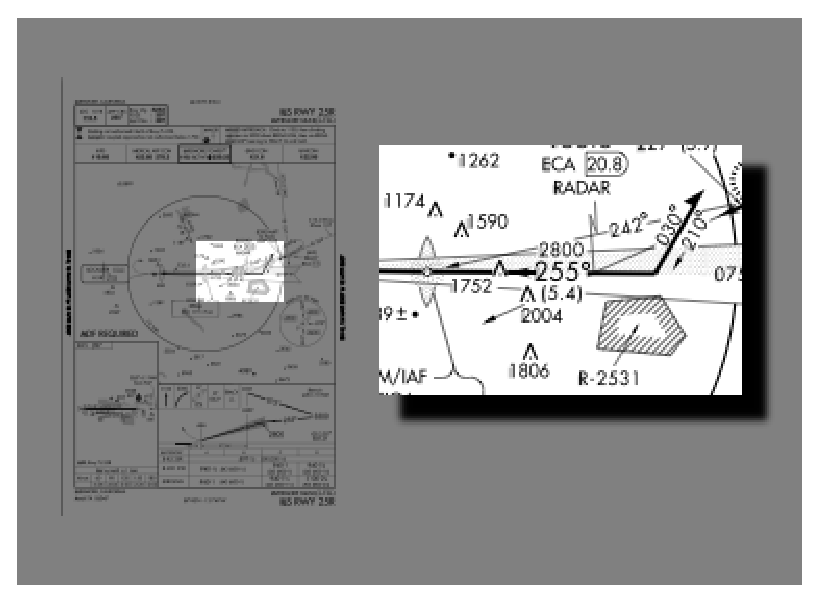
\includegraphics[width=7cm]{img/PT}
    \caption{Livermore ILS procedure turn}
    \label{fig:PT}
  \end{center}
\end{figure}

Hmmm.  I mentioned ``right altitude'', but how do we know that is?
That's down below, in the profile view (the yellow part of Figure
\ref{fig:big_plate}).  You can see that at the top is the LOM, our
IAF.  Now follow the arrows.  After the IAF, we head out at
075$^\circ$.  During the procedure turn we can descend to 3300 feet,
but \emph{no lower} (that's what the line \emph{under} the 3300
means).  After we finish our procedure turn and are heading back at
255$^\circ$, we can descend to 2800 feet, but \emph{no lower}, until
we intercept the glide slope.

One thing the instrument approach procedure does \emph{not} tell you
is the length of the procedure turn.  The only constraint is that you
must not fly more than 10 nm away from the NDB.  You'll notice there's
a 10 nm circle drawn around it in the plan view, and a note in the
profile view saying ``Remain within 10 NM''.  They're not kidding.
So, since we fly at around 110 knots, two minutes on each leg is
reasonable --- two minutes at 075$^\circ$, and two minutes at
030$^\circ$.  On the way back we don't care about times --- we just
want to intercept 255$^\circ$.

So, after we pass REIGA, turn right to 075$^\circ$ and start your
timer.

\subsection{Chasing the Needle}

% EYE - list actions?: turn, start timer, start descent, track
% EYE - using --ndb=LV to set my initial position doesn't work,
%       because several NDBs have the same ident
% EYE - documentation should state whether options use magnetic or
%       true headings
% EYE - do --offset-distance and --offset-azimuth only work in
%       relation to a runway specification?

When we approached REIGA, we weren't particularly concerned about our
course --- we just aimed for REIGA.  Now, however, our course is
important.  We want to be flying directly away from REIGA \emph{on a
  course of 075$^\circ$}.

Now, in an ideal world, after we turned to 075$^\circ$, the ADF needle
would be pointed directly behind you (ie, we'd be on course).
Probably it isn't, so we need to adjust our course.  The key to
adjusting our course is ADF Rule 2.  If we've set the compass card
correctly, then the needle shows us the current NDB ``radial''.  If we
turn and fly until we intercept the 255 ``radial'', then turn to
075$^\circ$, we'll be right on course.

Figure \ref{fig:NDB_flying} shows what I mean.  In the figure, the
plane, flying along the green line, is initially off
course.\footnote{\emph{Way} off course, actually.  I've exaggerated
  the angles to make the explanation clearer.}  The heading is
correct, 075$^\circ$, but the station is at 225$^\circ$, not
255$^\circ$.  To correct this, we turn right (remembering to adjust
the ADF compass card).  As we fly on this new heading, we get closer
to the correct position, crossing the 235 and 245 ``radials'' (shown
in red).  Finally, when we the ADF needle points to 255$^\circ$, we
turn left to 075$^\circ$, and readjust the ADF compass
card.\footnote{You might be thinking ``Wouldn't it be nice if there
  was an ADF where the compass card rotated automatically?''  Well,
  such an ADF does exist, and it comes with its own acronym --- RMI
  (Radio Magnetic Indicator).} We are now on course.

\begin{figure}
  \begin{center}
    \includegraphics[width=10cm]{img/NDB_flying}
    \caption{Getting back on course}
    \label{fig:NDB_flying}
  \end{center}
\end{figure}

Of course, even when you get back on track, that won't be the end of
the story.  Your airplane drifts; your mind drifts; your compass
drifts; the wind pushes you around.  What you find is that you will be
constantly making little corrections.  That's okay, as long as we're
close.  And anyway, before long (2 minutes actually), we'll turn left
45$^\circ$ to 030$^\circ$ as part of our procedure turn, at which
point we'll just ignore the NDB anyway.  Sigh.  All that effort for
just 2 minutes.  Hardly seems worth it.

\subsection{FOOTO Time}

While you're flying outbound, take an occasional look at VOR2, tuned
to Manteca, and the DME.  Assuming the OBS is still at 229, and the
DME still tuned to N2, at some point the needle should center, meaning
you've crossed the 229 radial, and, if you're on course, at the same
time the DME should read 20.8.  How do I know that?  If you look at
the approach plate (Figure \ref{fig:big_plate}), you'll notice an
intersection, named FOOTO.  FOOTO is on the approach, and is defined
to be 20.8 DME from ECA.  Although this intersection is not strictly
necessary for us, it comes for free, and provides good confirmation of
our position both outbound and, later, inbound.

Depending on how fast you're flying, you'll probably pass FOOTO close
to the time your two minutes at 075$^\circ$ are up.  At the end of two
minutes, turn left 45$^\circ$ to 030$^\circ$.  We'll fly for another
two minutes on this heading.

\subsection{George III}

This leg is relatively uneventful, so we'll take advantage of the lull
in the action to descend to 3300.  Assuming you're using the
autopilot, you will need to do a few things:

\begin{enumerate}
\item If you're in altitude hold (ALT) mode, you need to get back into
  vertical speed (VS) mode.  Press the ALT button --- the ``ALT'' in
  the middle of the display should change to ``VS'', and your current
  vertical speed (probably 0) should be displayed momentarily on the
  right.
\item Click the DN button until you get a vertical speed of -500 feet
  per minute.
\item If you want to set the target altitude, like before, rotate the
  big knob on the right until ``3300'' shows up on the right side of
  the display.  ``ALT ARM'' should appear on the bottom.
\end{enumerate}

Note that if you're using the autopilot to descend, it will just push
the nose down, like a bad pilot, so the airplane will speed up.  We
want to go down, but we don't want to speed up, so we need to reduce
engine RPMs to keep the speed at 110 knots.  Later, when you level off
at 3300 feet, you'll have to increase power again.

If you're flying manually, then you just need to adjust the engine to
get the descent rate you want --- the plane should stay magically at
110 knots if it's already trimmed for 110.

\subsection{ILS Landings}

While descending, we also need to start considering how we're going to
intercept 255$^\circ$ on the way back and follow it down to the
runway.  You might think we're going to use the NDB like we did on the
outbound leg, but at this point, the NDB is not good enough.  This is
an ILS landing, a so-called ``precision'' landing, and an NDB is just
not precise enough.  It can get us close to the runway, but not close
enough.

So, we're going to switch over to our ILS system.  It is much more
accurate horizontally.  As well, it offers vertical guidance,
something which the NDB does not give at all.  And hey, it also gives
you something else to learn in our few remaining minutes so that you
don't get bored.

As with NDB and VOR navigation, the ILS system\footnote{See
  \url{http://en.wikipedia.org/wiki/Instrument_Landing_System} for
  more information.} has a transmitter (or \emph{transmitters} --- a
localizer \emph{and} a glide slope) on the ground, and a receiver and
a gauge in the aircraft.  The receiver, it turns out, is just a NAV
receiver, of which we have two.  The gauge is like a VOR indicator,
but it has an added glide slope indicator, which is a horizontal (you
hope) needle.  Like a VOR, the vertical needle shows whether you're
left or right.  The horizontal needle shows whether you're high or
low.  Our ILS gauge is our old friend VOR1.

As you might have guessed, the localizer has a frequency and ident
associated with it (there's no need to tune the glide slope
separately.  If you tune the localizer, you've tuned the glide slope).
This is shown on the approach plate in two places: at the top left
corner, and in the plan view by the runway (see Figure
\ref{fig:localizer}).  As we can see, the frequency is 110.5 MHz, and
the ident is I-LVK (\mdot\mdot\mspace \mdot\mdash\mdot\mdot\mspace
\mdot\mdot\mdot\mdash\mspace \mdash\mdot\mdash).

% I-LVK = ../.-../...-/-.-

\begin{figure}
  \begin{center}
    \includegraphics[width=7cm]{img/localizer}
    \caption{Livermore 25R localizer}
    \label{fig:localizer}
  \end{center}
\end{figure}

Tune NAV1 to 110.5, and check for the ident.  Sounds lovely, doesn't
it?  That localizer is going to save your bacon and get you out of
this interminable soup.  When you tuned into the localizer, you'll
also have noticed the ILS needles move.  And the OBS?  Well, it's
useless.  Try moving it.  No matter how you turn it, the needles don't
move in response.  That's by design.  A localizer is basically a VOR
with \emph{one} radial, the approach heading.  We don't care about any
others, so we don't need an OBS to declare interest in any others.  As
a reminder, though, move the OBS to 255, our desired heading.  This
will remind us where to point our nose.

\subsection{Intercepting the Localizer}

We're now ready to intercept the ILS localizer.  When the two minutes
on the 030$^\circ$ leg have passed, make your U-turn to the right to
210$^\circ$.  Soon after you complete your turn, the vertical
(localizer) needle on the ILS will begin to move.  And it will move
\emph{fast}, much faster than the ADF and VOR needles did.  A
localizer is 4 times as sensitive as a VOR, relatively small movements
of the aircraft make big changes in the needles.  You'll probably
overshoot, but don't worry, because we have around 5 or 10 minutes to
get things straightened out.

Just remember: don't chase the needles.  That mantra is now more
important than ever.  Those needles are sensitive --- if you just turn
left when the localizer needle is to the left and right when it's to
the right, you'll be flying like a drunken sailor.  If you're lucky,
the runway will be passing underneath you as you swing across the
track for the umpteenth time.  Luck, though, is something we should
not be relying on.  Determine on how the needles are moving before
making your move.

Now that you're heading back inbound at 255$^\circ$, slow to 75 knots,
drop a notch of flaps, and descend to 2800 feet (but no lower).  And
check for the inbound passage of FOOTO to confirm your position.  And
pat your head and rub your stomach.

\subsection{Intercepting the Glide Slope}

As we fly drunkenly towards the runway, cursing localizers and needles
and resolving never, ever to fly in such crappy conditions ever again,
don't forget to look at the horizontal needle, the glide-slope needle.
At the start it was high above us, because we were actually under the
glide slope.  But as we levelled out at 2800, the glide slope started
coming ``down'' to us.  Eventually, you should see the needle start to
move down.  When the needle is horizontal, that means you're on the
glide slope.  You won't be for long, though, unless you start
descending.

What's a good rate?  It depends on our groundspeed.  In our case,
we're going at 75 knots (there's almost no wind, so our airspeed and
groundspeed are the same), and it turns out that we need to descend at
around 400 feet per minute.  With the autopilot, that's pretty easy
--- just dial in -400, and you're set (but remember to reduce power to
keep our speed at 75 knots, or you'll hit the runway going pretty
fast, and be prepared to adjust things if you drift above or below the
glide slope).

Without the autopilot, it's also pretty easy --- just reduce power.
How much?  In this case, with our plane, to around 1600 RPM.  Again,
it depends on many things --- plane, elevation, winds, weight,
\ldots{}, so you'll have to adjust things if you see the glide-slope
needle start to move up or down.  Like the localizer needle though,
\ldots{} (are you ready?)  DON'T CHASE IT.  Watch how it's moving,
then make your adjustment.

Since we're on final approach, you might want to drop a second notch
of flaps.  This will affect your trim, and you'll have to adjust power
a bit as well.

Soon after we intercept the glide slope, we should pass over the outer
marker.  Several things will happen more or less simultaneously, all
of which confirm your position:

\begin{enumerate}
\item You'll hear a continuous series of dashes.
\item The blue light above COMM1 will flash.
\item The ADF needle will swing around.
\end{enumerate}

\subsection{Touchdown, Almost}

After all the excitement of the procedure turn, it will seem like a
long way down to the runway from the outer marker.  There's not much
to do but stare at those needles.  In fact, you'll probably stare at
them like you've never stared at them before.  Take a look around at
the other gauges too, though --- they have useful things to tell you.
Is our airspeed okay?  We don't want to stall.  RPMs about right?  If
flying manually, you'll want to constantly check the attitude
indicator and directional gyro.  This being a simulator, we don't have
to worry about oil pressure and engine temperature, but you might want
to glance over there anyway, just to get into the habit.  And I hope
you've done things like set the mixture to full rich (you did lean it
out while cruising, didn't you?).

\subsection{Touchdown, Not}

% EYE - a nice 1/2 symbol?

Although ILS approaches can get us close to the runway, closer than
VFR, NDB, or VOR approaches can, we still need \emph{some} visibility
to land,\footnote{Well, unless it's a Category III ILS approach.} so
we need a way to decide if landing is possible or not.  That's what
the landing minimums section of the procedure plate is for (coloured
green in Figure \ref{fig:big_plate}).  In the category labelled
``S-ILS 25R'' (that's us), you'll see ``597-1/2 200(200-1/2)''.  This
tells us that we can track the glide slope down to an altitude of 597
feet (200 feet above the runway).  At 597 feet we make our decision
--- if we can't see the runway, then we have to execute a missed
approach.  597 feet is our \emph{decision height} (DH).

In addition to the altimeter, this particular approach also has
another indication that we're close --- a middle marker (MM).  This
marker will sound --- in this case, a dot dash series --- and the
yellow light above COMM1 will flash.  Passage over the middle marker
should coincide with reaching decision height.\footnote{As you may
  have guessed, the remaining, white, light above COMM1 indicates
  passage of the inner marker.  Our approach doesn't have one, but San
  Fransisco's runway 28R does.  While passing over it, you should hear
  a rapid, high-pitched series of dots.}

So, what if you can't see the runway at decision height?  As you might
have expected, just as you can't land willy-nilly, you can't just go
around willy-nilly.  There's a Procedure.  A Missed Approach
Procedure.  This is shown in several places on the approach plate (see
Figure \ref{fig:MAP}): At the top, where it says ``MISSED APPROACH'',
in the plan view, where you can see a dashed arrow coming off the end
of the runway and a dashed oval on the right, and in the profile view,
where a series of boxes shows graphically what to do.  In our case,
these all tell us to:

\begin{enumerate}
\item Climb straight ahead to 1100 feet
\item Make a climbing right turn to 3000 feet
\item Fly to REIGA
\item Fly outbound from REIGA at 062$^\circ$
\item Fly a holding pattern at the TRACY intersection
\end{enumerate}

\begin{figure}
  \begin{center}
    \includegraphics[width=7cm]{img/MAP}
    \caption{Missed approach procedure}
    \label{fig:MAP}
  \end{center}
\end{figure}

The holding pattern, as you might have guessed, is a place where you
can ``park'' while sorting things out, and has its own set of
procedures and techniques which we won't go into here, because
\ldots{}

\subsection{Touchdown}

In our ideal simulator world, you probably won't have to execute a
missed approach.  Assuming you stayed on the glide slope, you should
have popped out of the murk at 750 feet, a whole 153 feet above the
decision height, and with 1 mile visibility, the runway should have
been in view soon after.  With the runway in sight, you could then
turn wildly to get on course\footnote{Remembering, of course, to
  disengage the autopilot.}  (it's very hard to be lined up perfectly)
and land ``normally'' (which for me involves a lot of bouncing around
and cursing).  Park the plane, then stagger out of the cockpit and
have another hamburger!

\begin{figure}
  \begin{center}
    \includegraphics[width=10cm]{img/DH_plane_clipped}
    \caption{At decision height, runway in view.  We're going to live!}
    \label{fig:DH_plane_clipped}
  \end{center}
\end{figure}

% EYE - better navigational information websites?

\section{Epilogue}

%% There is so much more to IFR flying than what I've just presented.  In
%% FlightGear, we're all alone in our silent world and can do whatever we
%% want.  In the real world, you need to file flight plans, get them
%% approved, watch out for traffic, stay in contact with ATC, accept
%% instructions (which may deviate from your oh-so-carefully-conceived
%% flight plan), \ldots{}, the list goes on and on.  As if flying wasn't
%% hard enough, with ATC you need to fly and talk at the same time!

That was a lot of information in a short time, a rather brutal
introduction to ILS flying.  Hopefully, instead of turning you off, it
has whetted your appetite for more, because there \emph{is} more.
Some of the major issues I've ignored are:

\begin{description}
\item[Wind] This is a big one.  Flying IFR in a crosswind affects
  everything you do, and you need to be aware of it or your navigation
  will suffer.
\item[Flying without the autopilot] George tries his best, but he's
  not completely trustworthy.  You have to be prepared to go it
  alone.
\item[DG precession] The directional gyro in the c172p is not perfect.
  Over time, the values it gives you are less and less reliable --- it
  \emph{precesses}.  It needs to be periodically calibrated against
  the compass (using the OBS knob on the DG to adjust it).
\item[IFR charts] We used sectionals, which are really intended for
  VFR flight.  There are a whole set of charts devoted exclusively to
  IFR flight.
\item[ATC] The other people out there need to know what you're doing.
  As well, they'll probably tell you what to do, including to ignore
  the approach plate you so fastidiously studied.
\item[SIDs/DPs, Airways, and STARs] This tutorial introduced IAPs,
  which are standard ways to make approaches.  In IFR flight, there
  are standard ways to \emph{leave} airports (Standard Instrument
  Departures, \emph{SIDs}, or Departure Procedures, \emph{DPs}),
  standard ways to travel \emph{between} airports (airways), and
  standard ways to go from airways to IAPs (Standard Terminal Arrival
  Routes, \emph{STARs}).
\item[Holding Patterns] Most missed approaches end in a holding
  pattern somewhere, so you'd better know how to fly them.
\item[GPS] Our Cessna doesn't have a GPS, but nowadays most small
  planes do, and GPS is rapidly replacing radio-based navaids.
\end{description}

If you want to learn more, try the following resources:

\begin{itemize}
\item \textit{Flight Simulator Navigation}, written by Charles Wood.
  It covers everything from basic navigation to ILS approaches, with
  lots of examples and practice flights to improve your skills.
  Everything is linked together by an entertaining storyline in which
  you are the pilot for a fictional charter service.

  Two caveats, though.  First, it is Microsoft Flight Simulator-based,
  so you'll have to translate into ``FlightGear-ese'' as appropriate.
  Second, it is a bit out of date, and things in the real world have
  changed since it was written.  NDB beacons have been decommissioned,
  new approaches have replaced old ones --- even an airport has
  disappeared (!).  Treat this as a learning opportunity.  You'll get
  better at finding more up to date information, and learn not to
  blindly trust your charts, just as you have learned not to blindly
  trust your instruments.

  \url{http://www.navfltsm.addr.com}

\item If you're \emph{really} keen and want to hear it straight from
  the horse's mouth, there's the official \textit{FAA Instrument
    Flying Handbook}.  It's big and detailed, and there's \emph{no}
  interesting storyline in which you're a pilot for a fictional
  charter service.  It can be downloaded as two PDF files.

  \url{http://www.faa.gov/library/manuals/aviation/instrument_flying_handbook}

\item If you'd like practice deciphering what the instruments are
  telling you, without the bother flying (or even virtual flying), you
  can try \textit{luizmonteiro.com}, which has Flash tutorials of
  various instruments, including a VOR and an ADF.

  \url{http://www.luizmonteiro.com/Learning.aspx}

\item Another simulated instrument site is \textit{Tim's Air
  Navigation Simulator}.  It has a Java applet that simulates a plane
  flying in the vicinity of two navaids.  The simulation allows you to
  use different kinds of instruments and navaids, so you can see their
  behaviour, and the advantages and disadvantages of each.

% EYE - trailing slash?

  \url{http://www.visi.com/~mim/nav/}

\item If it's navigation information you're after, an excellent site
  is \textit{AirNav.Com}, which I've used extensively in the course of
  this tutorial.  It has detailed airport, navaid, and fix
  information, and links to IAPs.  Unfortunately, the information is
  only for the USA.

  \url{http://www.airnav.com}

\item Another source of airport and navaid information is
  \textit{World Aero Data}.  Its information isn't as detailed as
  AirNav's, but it is international.

  \url{http://worldaerodata.com}

\item \textit{FlightSim.Com} has a very informative series of articles
  entitled ``How To \ldots{} Use Approach Plates''.  It starts with a
  \emph{very, very} dense tutorial on how to read an approach plate,
  then follows with a set of approaches at Kodiak, Alaska.  These are
  an excellent supplement to the approaches given in Charles Wood's
  \textit{Flight Simulator Navigation} (see above).

  Most interesting, though, is section two --- ``Dangerous
  Approaches.''  Approaches at six airports around the world, from
  Penticton, BC to Kathmandu, Nepal, are described.  Fly them if you
  dare!

  Warning --- the series is even more Microsoft Flight
  Simulator-centric than Charles Wood's, and some of it is out of date
  (some outside links are broken, and some of the approaches have
  changed).

  \url{http://www.flightsim.com/cgi/kds?$=main/howto/plate/linkpage.htm}

% Add?
%
% http://www.acukwik.com/
%
% More airport and flying information

% Add?
%
% http://www.fsstation.com/tutorials/approachplates.html
%
% Another short tutorial on approach plates.

% Add?
%
% http://www.fsstation.com/tutorials/dangerous-airports-approaches.html
%
% Five approaches with short descriptions.

% Add?
%
% http://www.flightsim.com/cgi/kds?$=main/howto/glass/glass.htm
%
% An explanation of glass cockpits.  It's pretty good, but still
% leaves a fair bit unexplained.

% Add?
%
% http://www.fsstation.com/tutorials/boeing-pmdg-737ng.html
%
% A complete flight in a nice 737 simulation.  Has descriptions of
% using the Flight Management Computer (FMC), and many pictures of the
% Primary Flight Display (PFD) and Navigation Display (ND).  Often it
% talks about the ``FMA'' (Flight Mode Annunciator), which are the
% labels at the top of the PFD.

% Add?
%
% http://www.united-virtual.com/classes/index.html
%
% The first entry in a series about flying with another virtual
% airline (United, in this case).  It's geared totally toward big
% airliners, so offers a different perspective on things.  It's a nice
% introduction, providing useful information without expecting you to
% know everything already.

% Add?
%
% http://www.jeppesen.com/wlcs/index.jsp?section=resources&content=publications_aopa.jsp
%
% A page with pointers to 3 sets of publications: 'Jeppesen Electron
% Chart Clinic, 'The NavData Chart Clinic', and 'The Chart Clinic'.
% It's all Jeppesen specific of course, but the 'Chart Clinic' series
% looks like it may be generally useful.

\item Also from \textit{FlightSim.Com} is ``Golden Argosy'', a
  description of a flight from New York to Rome by Tony Vallillo, an
  American Airlines 767 captain.  It gives some interesting
  information about navigation that doesn't appear in the other sites
  mentioned here, such as the North Atlantic Tracks.  However, its
  main appeal is that it gives a good answer to the question ``What's
  it \emph{really} like to be a pilot?''  The author's love of flying
  is evident throughout the article.

\url{http://www.flightsim.com/cgi/kds?$=main/feature/argosy1.htm}

\item For those who are interested in the ATC side of things, and want
  information from an authoritative source, check out Michael Oxner's
  ``Aviation Topic of the Week'', a series of articles about flying
  ``in many types of airspaces in many situations.''  Michael Oxner is
  a professional controller and private pilot who obviously can't get
  enough of airplanes, because in his spare time he's also an on-line
  controller with VatSim.  Particularly interesting are a set of
  articles describing a complete IFR flight and a complete VFR flight.

  \url{http://bathursted.ccnb.nb.ca/vatcan/fir/moncton/WeeklyTopics/WeeklyTopicIntro.html}

%% \item Holds are mentioned frequently, but rarely described (viz., this
%%   tutorial).  A good description can be found at:

%%   \url{http://www.flightsim.com/cgi/kds?$=main/howto/hold2.htm}

\item Freeworld Airways is a virtual airline.  Their ``flight school''
  has lots of useful information about navigation (including holding
  patterns, SIDs, and STARs), ATC and communication, and weather.

  Also interesting are two example flights, one in Europe and one in
  North America, showing the interaction between pilot and ATC.

  \url{http://www.freeworld-airways.net/main/training.php}

\end{itemize}
